\chapter{Getting Started}
\label{chap:starting}

\section{Hello Proofs}

The first and basic step in using Why3 is to write a suitable input
file. When one wants to learn a programming language, you start by
writing a basic program. Here we start by writing a file containing a
basic set of goals. 

Here is our first Why3 file, which is the file
\texttt{examples/hello\_proof.why} of the distribution.
\verbatiminput{../examples/hello_proof.why} Any declaration must occur
inside a theory, which is in that example called TheoryProof and
labelled with a comment inside double quotes. It contains three goals
named $G_1,G_2,G_3$. The first two are basic propositional goals,
whereas the third involves some integer arithmetic, and thus it
requires to import the theory of integer arithmetic from the Why3
standard library, which is done by the \texttt{use} declaration above.

We don't give more details here about the syntax and refer to
Chapter~\ref{chap:syntax} for detailed explanations. In the following,
we show how this file is handled in the Why3 GUI
(Section~\ref{sec:gui}) then in batch mode using the \texttt{why3}
executable (Section~\ref{sec:batch}). 


\section{Getting Started with the GUI}
\label{sec:gui}

The graphical interface allows to browse into a file or a set of
files, and check the validity of goals with external provers, in a
friendly way. This section presents the basic use of this GUI. Please
refer to Section~\ref{sec:ideref} for a more complete description.

\begin{figure}[tbp]
  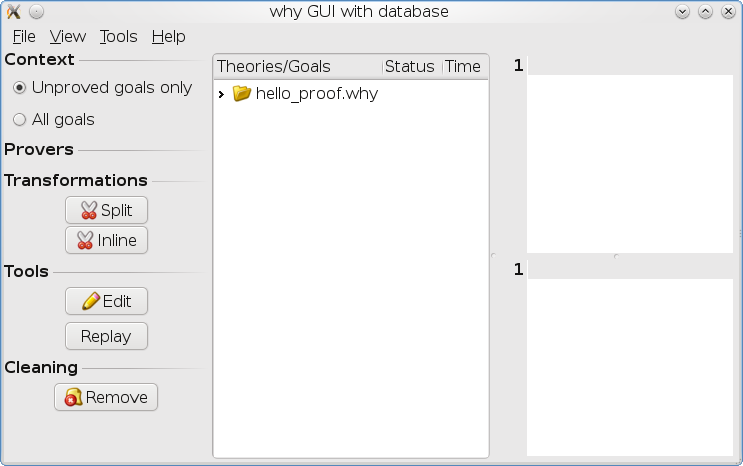
\includegraphics[width=\textwidth]{gui1.png}
  \caption{The GUI when started the very first time}
  \label{fig:gui1}
\end{figure}

The GUI is launched on the file above as follows.
\begin{verbatim}
why3ide hello_proof.why
\end{verbatim}
When the GUI is started for the first time, you should get a window
which look like the screenshot of Figure~\ref{fig:gui1}. First of all,
the left row is a tool bar which provide different actions to apply on
goals. In this case, the section ``Provers'' is empty, which means
that you did not perform prover detection yet. You should do it now
using the menu \textsf{File/Detect provers}. Second, the middle part
is a tree view that allows to browse inside the theories. Initially,
the item of this tree are closed. You should now expand this view
using the menu \textsf{View/Expand all} or its shortcut
\textsf{Ctrl-E}. This should result is something like the screenshot of Figure~\ref{fig:gui2}.

\begin{figure}[tbp]
  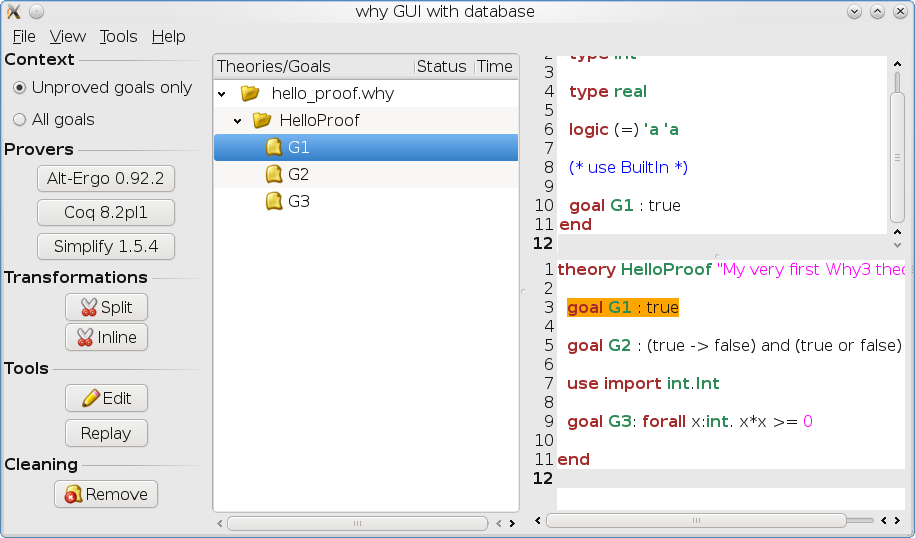
\includegraphics[width=\textwidth]{gui2.png}
  \caption{The GUI with provers detected and tree view expanded}
  \label{fig:gui2}
\end{figure}

In the tree view, we have now a strctured view of the file: this file
contains one theory, itself containg three goals. In
Figure~\ref{fig:gui2}, we also clicked on the row corresponding to
goal $G_1$. The \emph{task} associated with this goal is then
displayed on the top right, and the corresponding part of the input
file is shown on the bottom right part.

Notice also that three provers where detected, and are now shown as
button in the ``provers'' section of the left toolbar. In that case,
detected provers are Alt-Ergo~\cite{ergo}, Coq~\cite{CoqArt} and
Simplify~\cite{simplify05}. 

\subsection{Calling provers on goals}

You are now ready to call these provers on the goals. Whenever you
click on a prover button, this prover is called on the goal selected
in the tree view. You can even select several goals at a time, either
by using multi-selection (typically by clicking while pressing the
\textsf{Shift} or \textsf{Ctrl} key) or by selecting the parent theory
or the parent file. Let us now select the theory ``HelloProof'' and
click on the \textsf{Simplify} button. After a short time, you should
get the display of Figure~\ref{fig:gui3}.

\begin{figure}[tbp]
  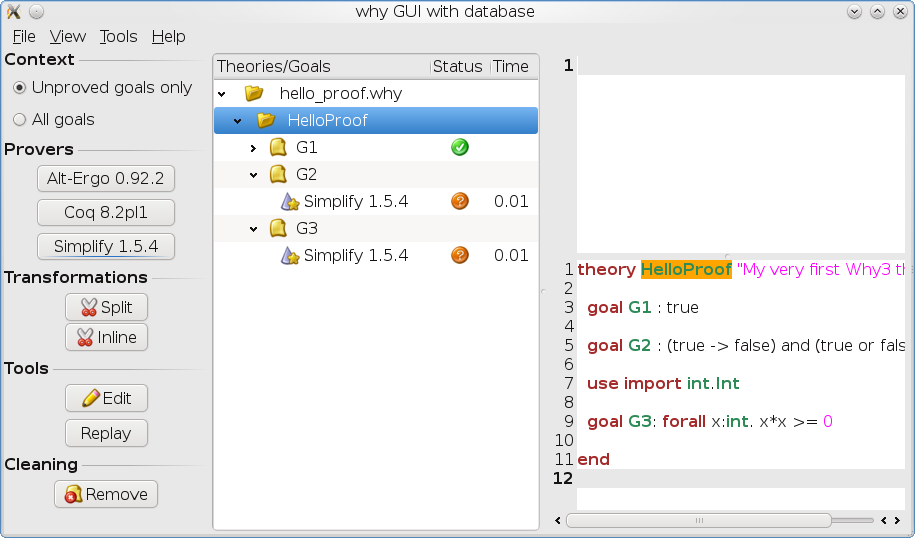
\includegraphics[width=\textwidth]{gui3.png}
  \caption{The GUI after Simplify prover is run on each goal}
  \label{fig:gui3}
\end{figure}

The row corresponding to goal $G_1$ is now closed, and marked with
green ``checked'' icon in the status column. This means that the goal
is proved by the Simplify prover. On the contrary, the two other goals
are not proved, they are mark with an orange question mark.

You can immediately attempt to prove the remaining goals using another
prover, {\eg} Alt-Ergo, by clicking on the corresponding button. The
goal $G_3$ should be proved now, but not $G_2$. 

\subsection{Applying transformations}

Instead of calling a prover on a goal, you can apply a transformation
to it.  Since $G_2$ is a conjunction, a possibility is to split it
into subgoals. You can do that by clicking on the \textsf{Split}
button of section ``Transformations'' of the left toolbar. Now you
have two subgoals, and you can try again a prover in them, for example
Simplify. Assuming we expand everything again, you should see now what
is displayed on Figure~\ref{fig:gui4}.

\begin{figure}[tbp]
  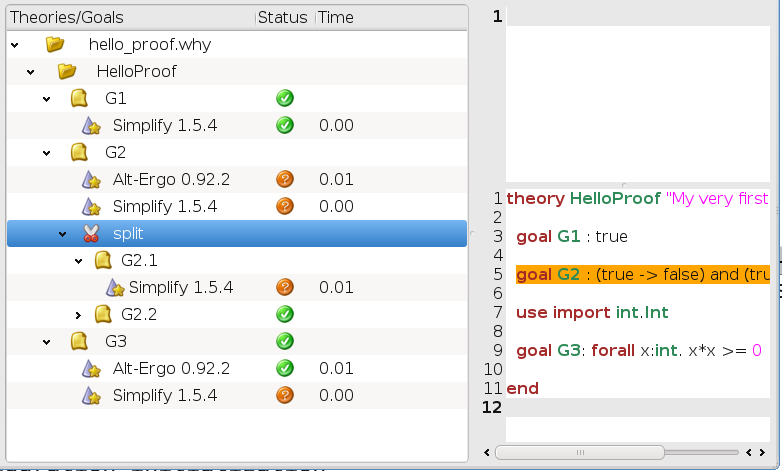
\includegraphics[width=\textwidth]{gui4.png}
  \caption{The GUI after splitting goal $G_2$}
  \label{fig:gui4}
\end{figure}

The first part of goal $G_2$ is still unproved. As a last resort, we
can try to call the Coq proof assistant. The first step is to click on
the \textsf{Coq} button. A new sub-row appear for coq, and
unsurprisingly the goal is not proved by Coq either. What can be done
now is editing the proof: select that row and then click on the
\textsf{Edit} button in section ``Tools'' of the toolbar. This should
launch the Coq proof editor, which is \texttt{coqide} by default (see
Section~\ref{sec:ideref} for details on how to configure this). You get
now a regular Coq file fo fill in, as shown on Figure~\ref{fig:coqide}.
Please take care of the comments of this file. Only the part between
the two last comments can be modified. Moreover, these comments
themselves should not be modified at all, they are use to mark the
part you modify, in order to regenerate the file if the goal is
changed. 

\begin{figure}[tbp]
  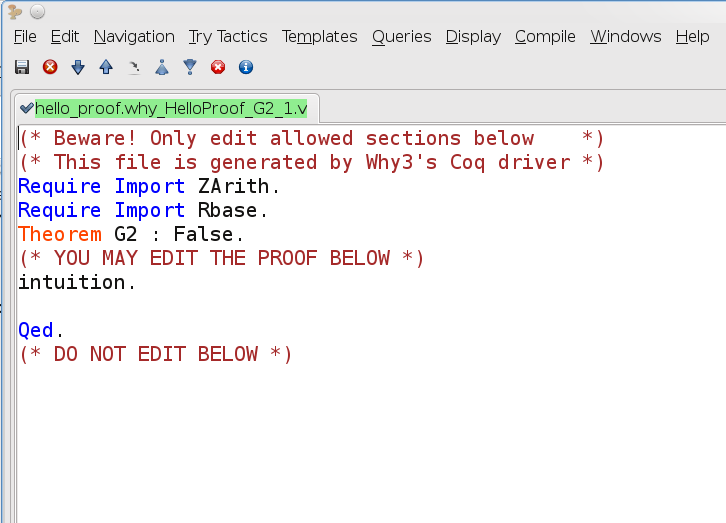
\includegraphics[width=\textwidth]{coqide.png}
  \caption{CoqIDE on subgoal 1 of $G_2$}
  \label{fig:coqide}
\end{figure}

Of course, in that particular case, the goal cannot be proved since it
is not valid. The only thing to do is to fix the input file, as
explained below.

\subsection{Modifying the input}

Currently, the GUI does not allow to modify the input file. You must
exit the GUI and modify the file by some editor of your choice. Let's assume we change the goal $G_2$ into
\begin{verbatim}
  goal G2 : (false -> false) and (true or false)
\end{verbatim}
Starting the IDE on the modified file and expanding everything with
\textsf{Ctrl-E}, we get the tree view shown on Figure~\ref{fig:gui5}.

\begin{figure}[tbp]
  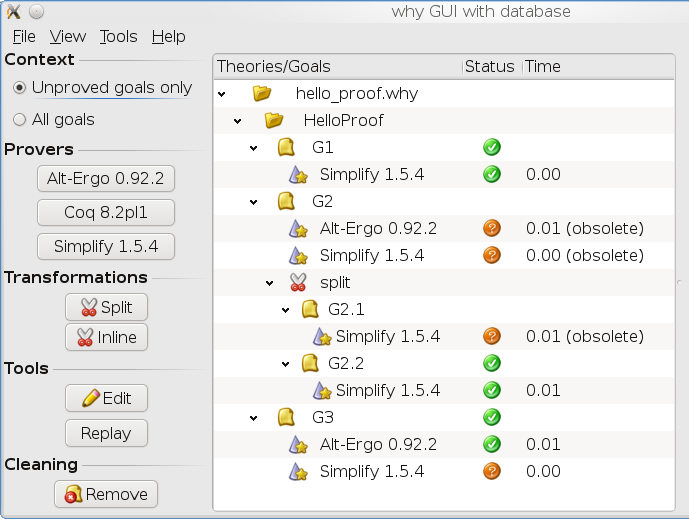
\includegraphics[width=\textwidth]{gui5.png}
  \caption{The GUI restarted after modifying goal $G_2$}
  \label{fig:gui5}
\end{figure}

The important feature to notice first is that all the previous proof
attempts and transformations where saved in some database. Then, for
all the goals that remain unchanged, the previous proofs are shown
again. For the parts that changed, the previous proofs attempts are
shown but marked with "(obsolete)" so that you know the results are
not accurate. You can now retry to prove all what remains unproved
using any of the provers.


\section{Getting Started with the Why3 Command}
\label{sec:batch}

The why3 command allows to check the validity of goals with external
provers, in batch mode. This section presents the basic use of this
tool. Refer to Section~\ref{sec:why3ref} for a more complete
description.

[TO BE COMPLETED]




%%% Local Variables:
%%% mode: latex
%%% TeX-PDF-mode: t
%%% TeX-master: "manual"
%%% End:
